\documentclass[conference]{IEEEtran}
\usepackage{graphicx}
\usepackage{booktabs}
\usepackage{url}
\usepackage[hidelinks]{hyperref}
\makeatletter\setlength{\@fptop}{0pt}\setlength{\@fpsep}{10pt}\makeatother
\hypersetup{pdfauthor={Tanmayi Shurpali, Santhoshkumar Chandrasekar, Praniti Sunil Kale, Mukul Sridar Haladhi},pdftitle={Time Travel Inside a Diffusion Model},pdfcreator={},pdfproducer={}}

\begin{document}

\title{Time Travel Inside a Diffusion Model:\\ Watching, Rewinding and Changing Stable Diffusion While It Paints}

\author{\IEEEauthorblockN{Tanmayi Shurpali, Santhoshkumar Chandrasekar, Praniti Sunil Kale, Mukul Sridar Haladhi}
\IEEEauthorblockA{IE 7615 Deep Learning for AI, Northeastern University, Boston, MA\\
Repository: \url{https://github.com/tanmayi123/from-words-to-worlds}}}

\maketitle

\section{Question}
A text-to-image model receives a whole sentence at once but paints it over many denoising steps, and it often leaves out an object the sentence names. We ask \emph{when} each word gets painted, whether a word that is about to be dropped can be seen coming, and whether going back to an earlier step can save it without losing the rest of the picture. Earlier work shows that cross-attention maps fix an image's layout in the first steps \cite{p2p}, aggregates those maps into per-word heatmaps \cite{daam}, and repairs neglected objects by boosting their attention \cite{aae}. Other work repairs a flawed image by resampling it \cite{resample} or by choosing a step from which to refine it \cite{stepsel}. To our knowledge, none of it measures, word by word and across a dataset, the step at which a word's position is settled or an object is lost, or what a repair costs the rest of the picture. We measure both on 2{,}000 COCO captions, test whether they predict which objects appear, and test repairs by rewinding the generation.

\section{Dataset}
We use the MS-COCO 2017 validation split \cite{coco}: 5{,}000 photographs and 25{,}004 captions after cleaning. COCO pairs every prompt with a real photo and with labels for 80 object categories, so we can check whether a named object appears. Cleaning repaired whitespace in 3{,}832 captions and dropped 10 duplicates; wording was not edited, and every caption fits the encoder's 77-token window. Images are converted to RGB (10 were grayscale), center-cropped to a square and resized to $512\times512$; the crop keeps 72\% of an average frame, and the 12 evaluation pairs that lose more than half are flagged for any per-image comparison. The 42 images with a short side under 256 pixels are left out of the sets below, since enlarging them blurs them. With one fixed seed, the eligible images are split into three disjoint sets: 2{,}000 image-caption test pairs, 500 development pairs for choosing settings such as guidance and checkpoints, and 2{,}000 further photos used only as the real reference for FID and KID. We add 200 stress prompts (word order, counting, colour binding). From the 118{,}287-image training split, a cleaned 3{,}000-image subset is used for LoRA fine-tuning \cite{lora}, and the split's captions train the first stage of the connector described below.

\section{Model}
We use the pretrained Stable Diffusion 1.5 latent diffusion model \cite{ldm}; its weights stay frozen except for LoRA adapters and the connector below. A prompt is padded or truncated to 77 tokens and encoded by the CLIP ViT-L/14 text Transformer \cite{clip} into a $77\times768$ matrix. A UNet denoises a $64\times64\times4$ latent over 20 to 50 steps, reading that matrix through cross-attention at every step; a VAE decodes the result. Our own sampling loop controls classifier-free guidance \cite{cfg}, the DDPM and DDIM samplers \cite{ddpm,ddim}, and attention recording. For each word we record its cross-attention heatmap at every step, aggregated over heads and layers as in DAAM \cite{daam}. A word \emph{commits} at the first step after which its heatmap keeps a Pearson correlation of at least 0.8 with its final layout (the mean map of the last five steps before the final one). Since Imagen found the text encoder mattered more than the UNet \cite{imagen}, we also compare encoders: BERT \cite{bert} and GPT-2 \cite{gpt2} token states reach the UNet through a small connector with 77 learned query slots, trained first on captions alone to reproduce CLIP's states and then on image-caption pairs, with an identically trained CLIP connector as the control.

\section{Evaluation}
Image quality: FID \cite{fid}, KID \cite{kid} and Inception Score \cite{is}, with FID and KID each beside the score the reference photos earn against the test photos at the same sample size. Sweeps of guidance scale and step count trace the trade-off between fidelity and diversity. Text alignment: CLIPScore \cite{clipscore}, object recall from two COCO-trained detectors of different design, and VQAScore \cite{vqascore} for actions and relations where compute allows. Settings are chosen on the development pairs only. Comparisons share captions and seeds, use three seeds for every headline comparison, and report bootstrap confidence intervals.

\section{Plan}
Milestone 2 measures commit steps on all 2{,}000 test captions, alongside the image-quality baseline and sweeps of guidance, step count and sampler (the noise schedule), and trains the connector's first stage so BERT and GPT-2 can drive the model. Milestone 3 intervenes. Our sampling loop can rewind a painting to any step and finish it again, so we ask when a missing object is lost for good, and whether going back can bring it in without losing the rest of the picture, compared with simply painting again from a new seed. The same loop drives Rewind, a viewer in which a reader scrubs through the steps, edits the sentence and branches the painting. From any step it can also play the painting forward several times to show its possible futures and the chance that each named object survives, a repainting idea used to probe diffusion models \cite{phase} and to correct them \cite{resample}. Milestone 3 also compares the text encoders through the connector, and fine-tunes with LoRA to paint objects from our first course project, judged by that project's classifier. The final report also covers ethics: biases inherited from COCO and the model's training data, and misuse of tools that paint specific real objects.

\section{Team}
Each member leads one area and all four review every result and write the reports. \emph{Tanmayi Shurpali}: image-quality evaluation (FID, KID, Inception Score against the real-photo floor), the guidance and step-count sweeps, and calibrating the object judges on real photos. \emph{Santhoshkumar Chandrasekar}: the data and text-to-embedding pipeline, the attention recorder and commit measure, and the rewind loop with its experiments and the Rewind viewer. \emph{Praniti Sunil Kale}: the evaluation sets, object labels and stress prompts, and the training-free encoder comparison. \emph{Mukul Sridar Haladhi}: LoRA fine-tuning, the encoder connector, and painting objects from our first course project.

\section{Sample tests}
\emph{Text to embedding.} All 25{,}004 captions are encoded once and cached. Images generated from the cached states are pixel-for-pixel identical to Stable Diffusion's own output (mean absolute difference 0 on a 0 to 255 scale). As a sanity check, CLIP ranks the correct photo first among all 5{,}000 for 35.5\% of captions and in the top five for 59.9\% (chance: 0.02\%).

\emph{Generation.} Fig.~\ref{fig:samples} shows five captions at 30 steps and guidance 7.5, generated from the cached states in 3.0~s per image on a laptop RTX 5070. In these 15 samples the named objects usually appear; actions and relations (\emph{flying}, one man \emph{serving} another, \emph{looking to his left}) mostly do not.

\emph{Word timing.} Fig.~\ref{fig:timelines} applies the commit measure to two prompts (recording leaves the images unchanged). The first prompt is our smoke test's one failure, reproduced at its original seed: no cat appears. \emph{Bench} commits at step 1 and \emph{cat} at step 14 of 20, by which point the only unclaimed region is a small patch at the bench's edge. When dog and cat both appear, both commit at step 3. The order holds at thresholds of 0.7 and 0.9. Late commits are not always fatal: \emph{man} commits at step 20 of 30 for the cyclist in Fig.~\ref{fig:samples} and still appears. Milestone 2 tests whether commit time predicts object recall across 2{,}000 captions, and Milestone 3 tests it by intervention.

\emph{Development pilot.} We ran both questions on the 500 development captions. Of 378 named objects that two detectors judge, the 36 that both miss commit later than the 342 they find: median step 13 against 5, AUROC 0.82 (95\% interval 0.74 to 0.89), and 0.82 when only objects of the same class are compared. A word's share of attention over the first three of 30 steps already separates them (AUROC 0.76). For 34 of these failures, painting again from a new seed brings the object back within four tries 85\% of the time but never keeps the picture, while going back to step 12 brings it back 41\% of the time and keeps the picture for 35\% of failures (perceptual distance under half that between two unrelated paintings of the caption).

\emph{Other directions.} We also fine-tuned the UNet with LoRA, which gave a small CLIPScore gain on 40 prompts; compared text encoders without training, where BERT trails CLIP; and recaptioned 100 test photos with a captioning model, where longer captions gave no detectable gain in the objects drawn.

\begin{figure*}[t]
\centering
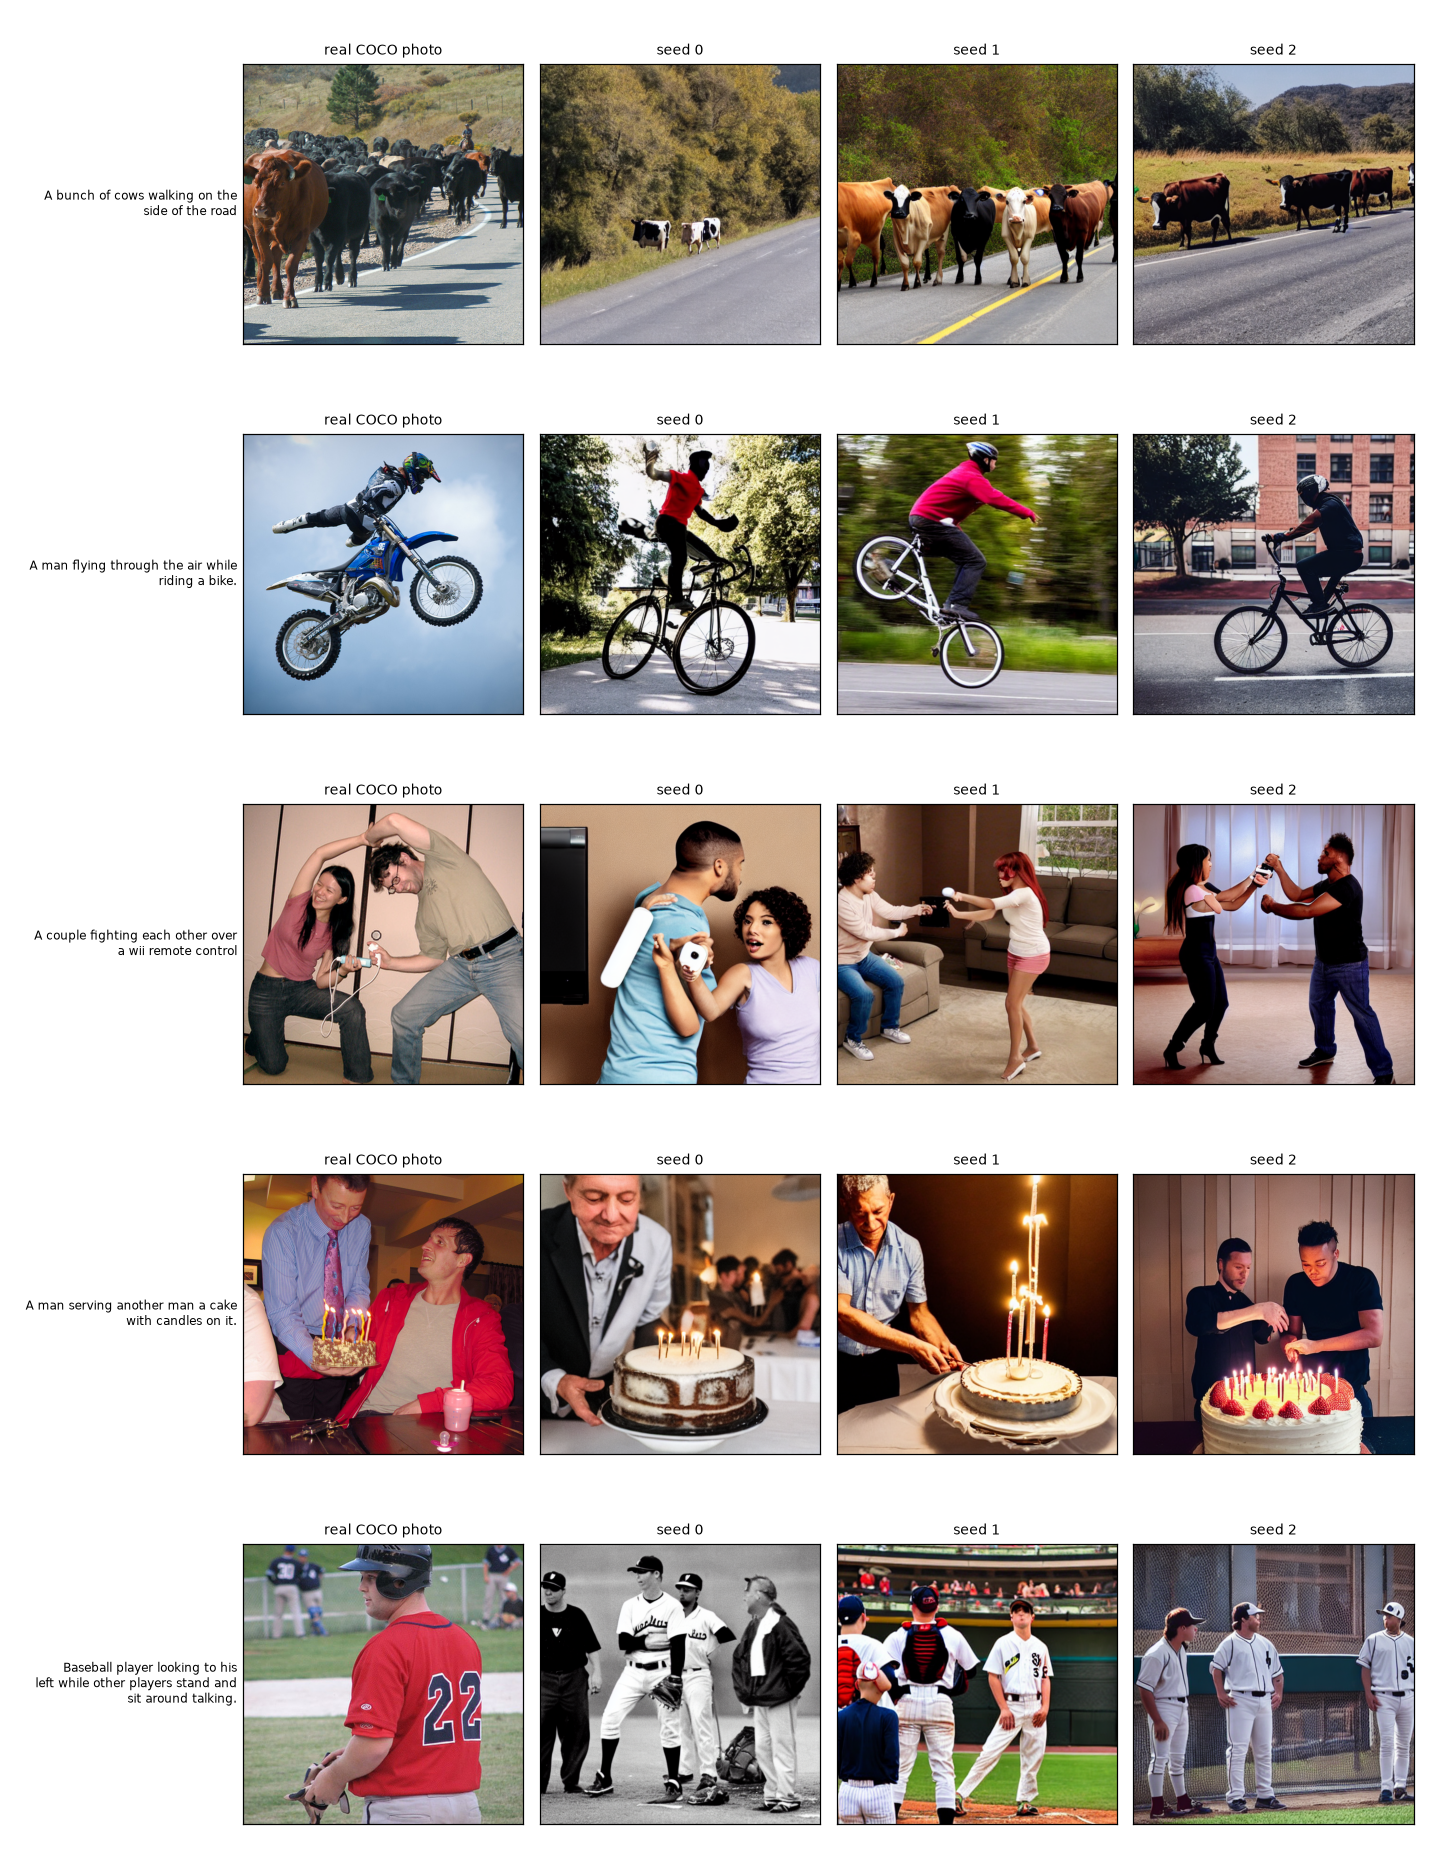
\includegraphics[width=0.56\textwidth]{../../Results/m1_pipeline/samples_grid.png}
\caption{Five COCO validation captions: the real photo, then seeds 0 to 2 generated from cached CLIP states (Stable Diffusion 1.5, 30 steps, guidance 7.5). Objects usually appear; the actions (\emph{flying}, \emph{serving}, \emph{looking to his left}) do not.}
\label{fig:samples}
\end{figure*}

\begin{figure*}[t]
\centering
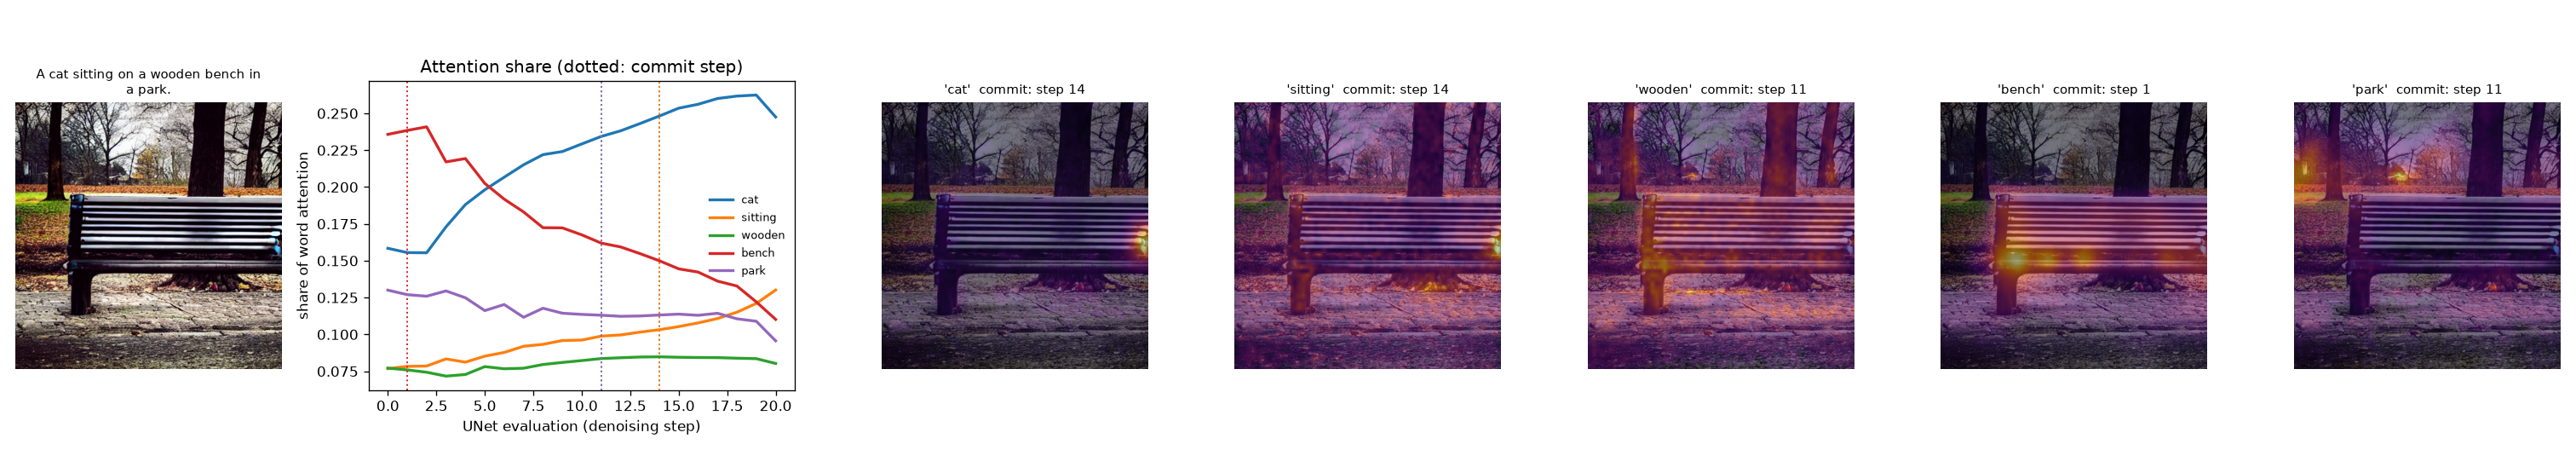
\includegraphics[width=\textwidth]{../../Results/m1_word_timelines/missing_cat_timeline.png}\\[2pt]
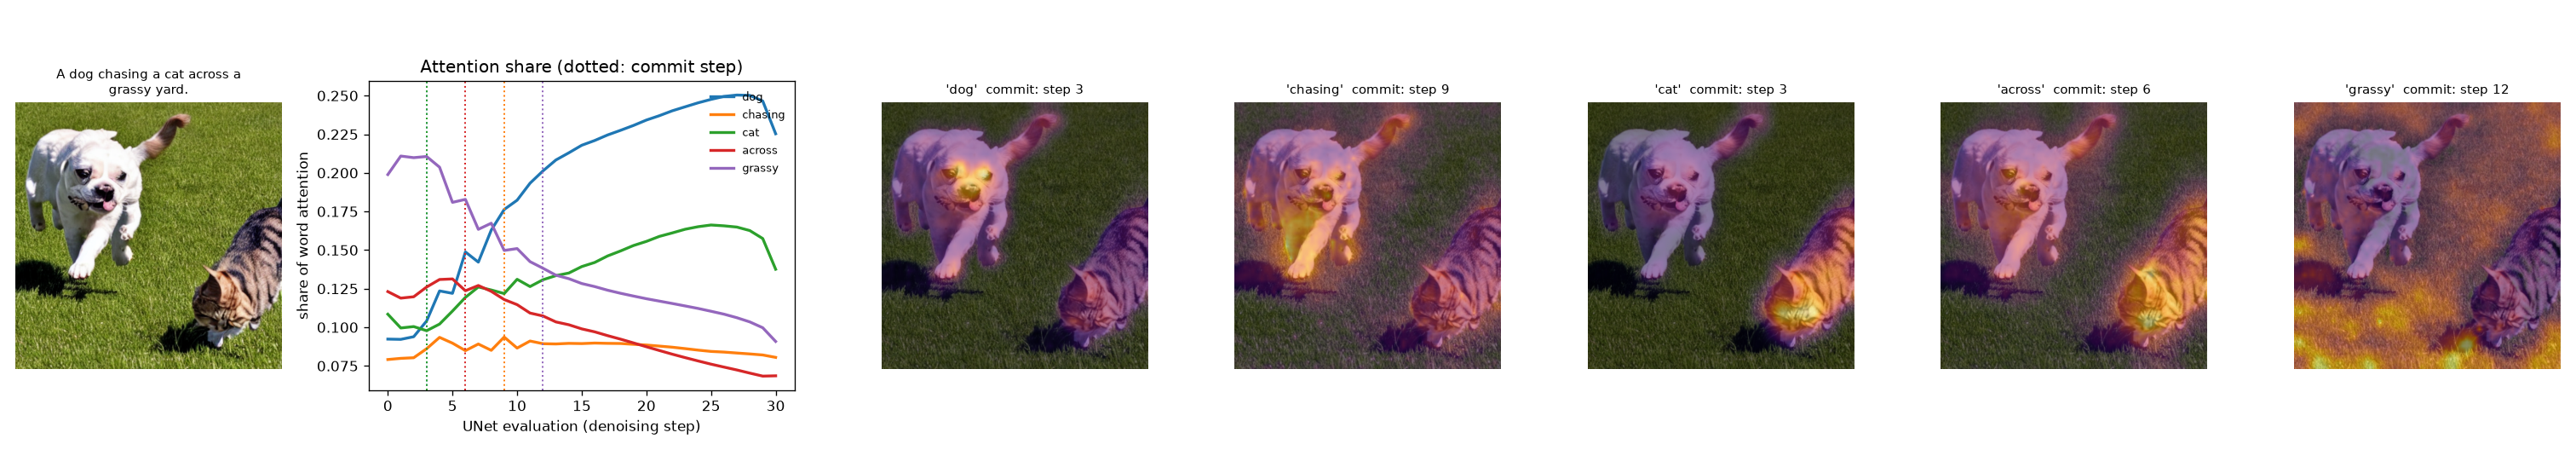
\includegraphics[width=\textwidth]{../../Results/m1_word_timelines/dog_chasing_cat_timeline.png}
\caption{Word timing on two prompts. Left to right: the generated image; each word's share of the attention given to the prompt's words (the start token, which takes about 89\% of all attention, is excluded) at every step, with a dotted line at each word's commit step; and where each word lands in the final image, with its commit step. Top (seed 2, 20 steps): \emph{cat} commits late and gets only a small patch at the bench's edge. Bottom (seed 0, 30 steps): dog and cat commit together and both appear.}
\label{fig:timelines}
\end{figure*}

\begin{thebibliography}{00}\footnotesize
\bibitem{p2p} A. Hertz, R. Mokady, J. Tenenbaum, K. Aberman, Y. Pritch, and D. Cohen-Or, ``Prompt-to-prompt image editing with cross attention control,'' in \emph{Proc. ICLR}, 2023.
\bibitem{daam} R. Tang et al., ``What the DAAM: Interpreting Stable Diffusion using cross attention,'' in \emph{Proc. ACL}, 2023.
\bibitem{aae} H. Chefer, Y. Alaluf, Y. Vinker, L. Wolf, and D. Cohen-Or, ``Attend-and-Excite: Attention-based semantic guidance for text-to-image diffusion models,'' \emph{ACM Trans. Graph.}, vol. 42, no. 4, 2023.
\bibitem{resample} Y. Liu, Y. Zhang, T. Jaakkola, and S. Chang, ``Correcting diffusion generation through resampling,'' arXiv:2312.06038, 2024.
\bibitem{stepsel} P. Grimal, H. Le Borgne, and O. Ferret, ``Text-to-image alignment in denoising-based models through step selection,'' arXiv:2504.17525, 2025.
\bibitem{coco} T.-Y. Lin et al., ``Microsoft COCO: Common objects in context,'' in \emph{Proc. ECCV}, 2014.
\bibitem{lora} E. J. Hu et al., ``LoRA: Low-rank adaptation of large language models,'' in \emph{Proc. ICLR}, 2022.
\bibitem{ldm} R. Rombach, A. Blattmann, D. Lorenz, P. Esser, and B. Ommer, ``High-resolution image synthesis with latent diffusion models,'' in \emph{Proc. CVPR}, 2022.
\bibitem{clip} A. Radford et al., ``Learning transferable visual models from natural language supervision,'' in \emph{Proc. ICML}, 2021.
\bibitem{cfg} J. Ho and T. Salimans, ``Classifier-free diffusion guidance,'' arXiv:2207.12598, 2022.
\bibitem{ddpm} J. Ho, A. Jain, and P. Abbeel, ``Denoising diffusion probabilistic models,'' in \emph{Proc. NeurIPS}, 2020.
\bibitem{ddim} J. Song, C. Meng, and S. Ermon, ``Denoising diffusion implicit models,'' in \emph{Proc. ICLR}, 2021.
\bibitem{imagen} C. Saharia et al., ``Photorealistic text-to-image diffusion models with deep language understanding,'' in \emph{Proc. NeurIPS}, 2022.
\bibitem{bert} J. Devlin, M.-W. Chang, K. Lee, and K. Toutanova, ``BERT: Pre-training of deep bidirectional transformers for language understanding,'' in \emph{Proc. NAACL}, 2019.
\bibitem{gpt2} A. Radford, J. Wu, R. Child, D. Luan, D. Amodei, and I. Sutskever, ``Language models are unsupervised multitask learners,'' OpenAI technical report, 2019.
\bibitem{fid} M. Heusel, H. Ramsauer, T. Unterthiner, B. Nessler, and S. Hochreiter, ``GANs trained by a two time-scale update rule converge to a local Nash equilibrium,'' in \emph{Proc. NeurIPS}, 2017.
\bibitem{kid} M. Bi\'{n}kowski, D. J. Sutherland, M. Arbel, and A. Gretton, ``Demystifying MMD GANs,'' in \emph{Proc. ICLR}, 2018.
\bibitem{is} T. Salimans, I. Goodfellow, W. Zaremba, V. Cheung, A. Radford, and X. Chen, ``Improved techniques for training GANs,'' in \emph{Proc. NeurIPS}, 2016.
\bibitem{clipscore} J. Hessel, A. Holtzman, M. Forbes, R. Le Bras, and Y. Choi, ``CLIPScore: A reference-free evaluation metric for image captioning,'' in \emph{Proc. EMNLP}, 2021.
\bibitem{vqascore} Z. Lin et al., ``Evaluating text-to-visual generation with image-to-text generation,'' in \emph{Proc. ECCV}, 2024.
\bibitem{phase} A. Sclocchi, A. Favero, and M. Wyart, ``A phase transition in diffusion models reveals the hierarchical nature of data,'' \emph{Proc. Natl. Acad. Sci. USA}, 2025.
\end{thebibliography}

\end{document}
